\documentclass{beamer}

\usepackage[utf8]{inputenc}
\usepackage[T1]{fontenc}
\usepackage[francais]{babel}
\usepackage{textcomp}

\usetheme{Rochester} % or Luebeck, Boadilla, Pittsburgh
\setbeamertemplate{navigation symbols}{}

\title{Répartiteur de charge}
\author{%
  Clément \textsc{Delpech} \\
  Armel   \textsc{Mangean} \\
  Idrissa \textsc{Sokhona}
}
\institute{Universtié Pierre et Marie Curie}
\date{
  14 Mai 2013 
}

\begin{document}

  \begin{frame}
    \titlepage
  \end{frame}

  \begin{frame}
    \frametitle{Introduction}
    \framesubtitle{}
    \begin{block}{Qu'est ce c'est?}
      Le répartiteur de charge est une application permettant de répartir
      l'execution des progrmmes sur différentes machines situées sur le 
      réseau.
    \end{block}
    
    Objectifs :
    \begin{itemize}
       \item Optimiser l'utilisation des ressources disponibles
       \item Mettre en \oe{}uvre des connaissances aquises précédemment
       \item Aquérir une expérience pratique des systèmes répartis 
     \end{itemize}
  \end{frame}
  
  
  \begin{frame}
    \frametitle{Problématiques}
    \framesubtitle{}
    % Parite 1.2 (Compréhension des problèmes) du rapport
    \begin{itemize}
      \item Comment évaluer de la charge d'une machine?
      \item Comment définir la surcharge?
      \item Quelle tâche déplacer?
      \item Quelle machine choisir?
      \item Comment gérer les pannes?
    \end{itemize}
  \end{frame}
  
  \begin{frame}
    \frametitle{Topologie}
    \framesubtitle{}
      \begin{figure}[h!]
        \centering
        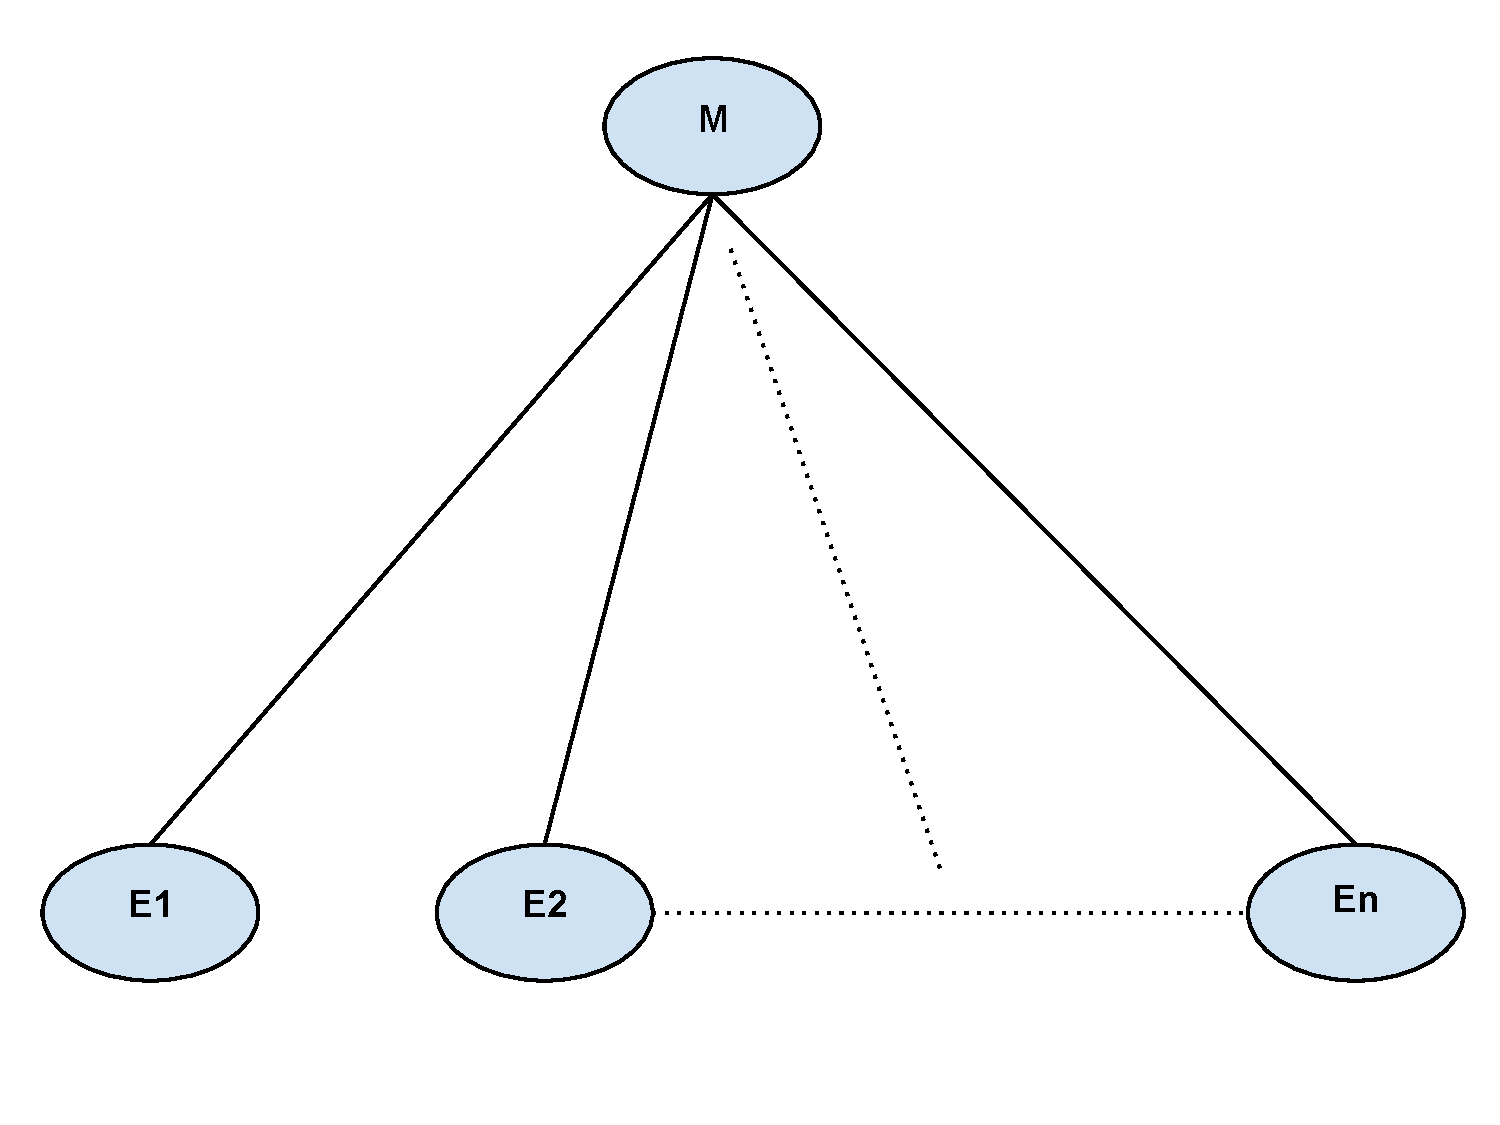
\includegraphics[scale=0.3]{img/topologie.pdf}
        \caption{Topologie du système de placement réparti}
      \end{figure}
  \end{frame}
  
  \begin{frame}
    \frametitle{Conception avec UML}
    \framesubtitle{Pourquoi UML?}
    \begin{block}{Pourquoi UML?}
      \begin{itemize}
        \item Mise en pratique des connaissances aquises
        \item Méthode de conception standardisé et largement répendue
        \item Procédure RPC $\approx$ Méthode UML
      \end{itemize}
    \end{block}
  \end{frame}
  
  \begin{frame}
    \frametitle{Conception avec UML}
    \framesubtitle{Exemple d'utilisation UML : diagramme de séquence}
      % TODO - Mettre un diagramme de séquence
  \end{frame}
  
  \begin{frame}
    \frametitle{Conception avec UML}
    \framesubtitle{Exemple d'utilisation UML : diagramme de classes}
      \begin{figure}[h!]
        \centering
        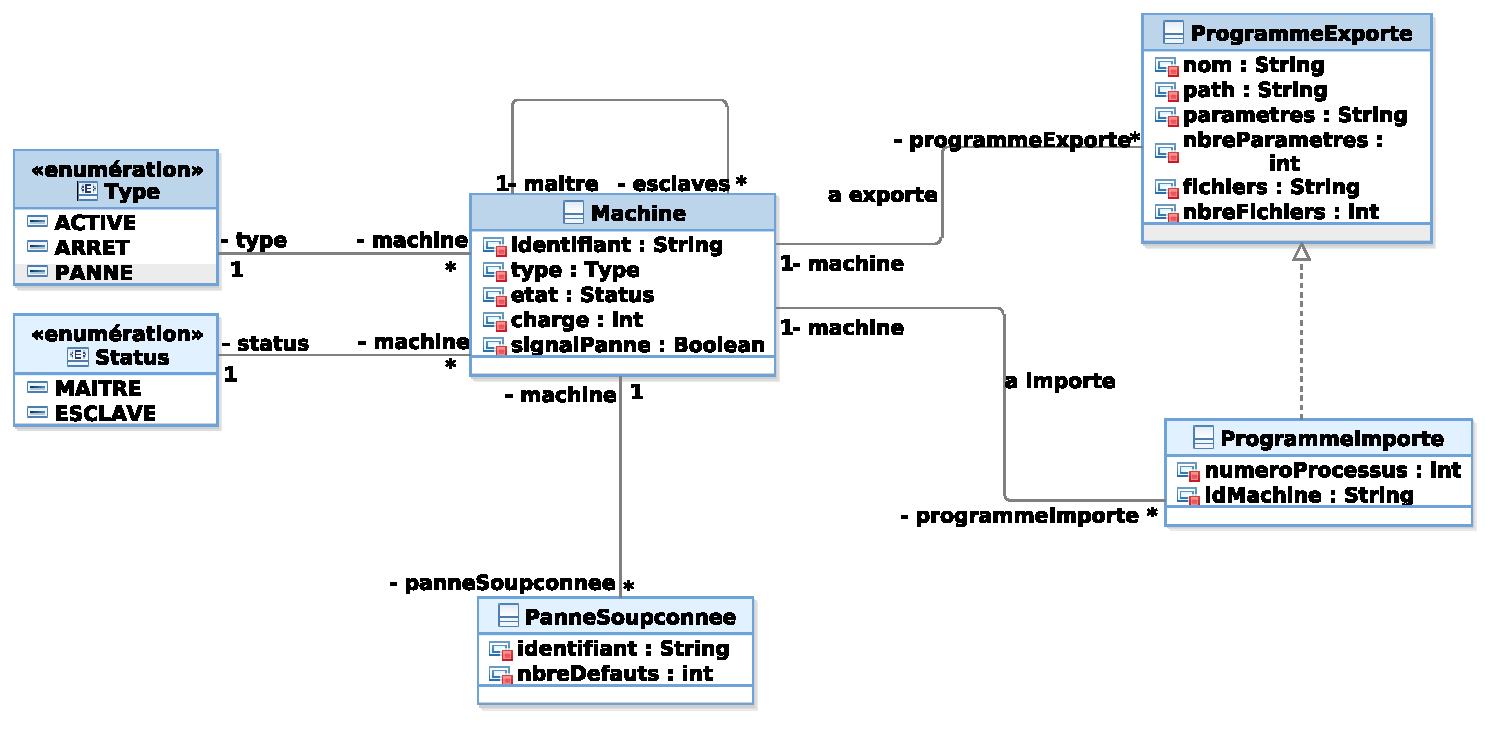
\includegraphics[scale=0.43]{img/analyse_dcl.pdf}
        \caption{Diagramme des structures}
      \end{figure}
  \end{frame}
  
  \begin{frame}
    \frametitle{Implementation}
    \framesubtitle{RPC, procédures distantes, procédures locales}
      \begin{itemize}
        \item Utilisation de RPC :
      \end{itemize}
  \end{frame}
  
  \begin{frame}
    \frametitle{Implementation}
    \framesubtitle{Quels problèmes rencontrés}
      \begin{itemize}
        \item 
      \end{itemize}
  \end{frame}
  
  \begin{frame}
    \frametitle{Utilisation}
    \framesubtitle{}
      
      Un interface simple, en ligne de commande. 
      \begin{block}{Les 5 commandes}
      \begin{description}
        \item[HELP] Affiche l'aide
        \item[EXECUTE] Exécute un programme
        \item[ADMIN] Affiche l'état du système 
        \item[QUIT] Quitte avec attente de terminaison des programmes 
        \item[KILL] Quitte sans attente
      \end{description}
      \end{block}
  \end{frame}
  
  \begin{frame}
    \frametitle{Tests}
    \framesubtitle{}
  \end{frame}
  
  \begin{frame}
    \frametitle{Améliorations possibles}
    \framesubtitle{}
    \begin{itemize}
       \item Algorithme de calcul de la charge
       \item 
    \end{itemize}
  \end{frame}
  
  \begin{frame}
    \frametitle{Conclusion}
    \framesubtitle{}
  \end{frame}
\end{document}
